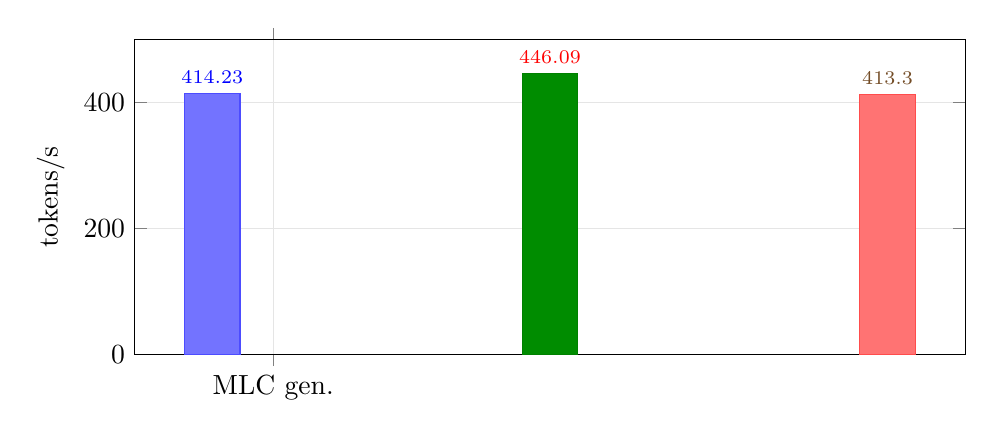
\begin{tikzpicture}
\begin{axis}[
    ybar,
    width=\linewidth,
    height=0.46\linewidth,
    ymin=0,
    ymax=500,
    ylabel={tokens/s},
    symbolic x coords={MLC gen.,MLC decode,vLLM gen.},
    xtick=data,
    nodes near coords,
    nodes near coords align={vertical},
    bar width=20pt,
    enlarge x limits=0.25,
    grid=major,
    major grid style={draw=black!10},
    every node near coord/.append style={font=\scriptsize},
]
\addplot+[fill=blue!55, draw=blue!70] coordinates {(MLC gen.,414.23)};
\addplot+[fill=green!55!black, draw=green!50!black] coordinates {(MLC decode,446.09)};
\addplot+[fill=red!55, draw=red!70] coordinates {(vLLM gen.,413.30)};
\end{axis}
\end{tikzpicture}
